\chapter{Background and Literature Review}\label{ch:problem}
%---------------------------------------------------------
\section{Preliminaries and Notation}\label{preliminaries}
This thesis uses the following notation, nomenclature, and fundamental equations of motion for fixed wing rigid body aerodynamics.

\subsection{Kinematics}
The following is the nomenclature that will be used to describe the kinematic equations.  Euler angles for pitch $(\theta)$, roll $(\phi)$, and yaw $(\psi)$ will have the units of radians.  The following Figure~\ref{fig:reference_frame} illustrates the \ac{NED} reference frame definitions used for body rotational rates about the $x$ axis $(p)$, $y$ axis $(q)$, and the $z$ axis $(r)$ as well as the body velocities in the $x$ axis $(u)$, $y$ axis $(v)$, and the $z$ axis $(w)$.

\begin{figure}[h!]
 \centering
  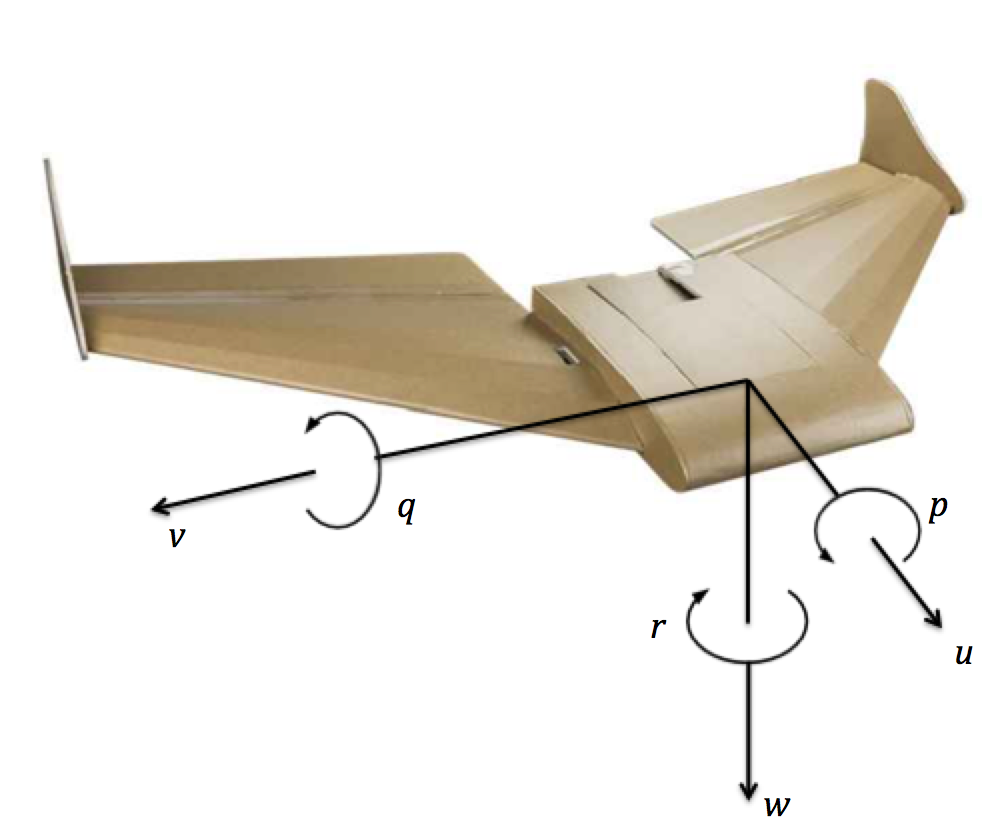
\includegraphics[width=0.65\textwidth]{body_frame_rotations.png}
  \caption{Reference frame - body rates and velocities}
  \label{fig:reference_frame}
\end{figure}

\subsection{First Order Model}
The following nomenclature will be used to illustrate the modeling of first order systems where $\dot{x}$ is the time derivative of the state, A is the Hurwitz matrix, B is the input matrix, and u is the input vector.
\begin{equation}
\dot{x}(t)=Ax(t)+Bu(t)
\end{equation}

\subsection{Second Order Model}


%---------------------------------------------------------
\section{Feedback vs Adaptive Control}

\begin{figure}[h!]
 \centering
  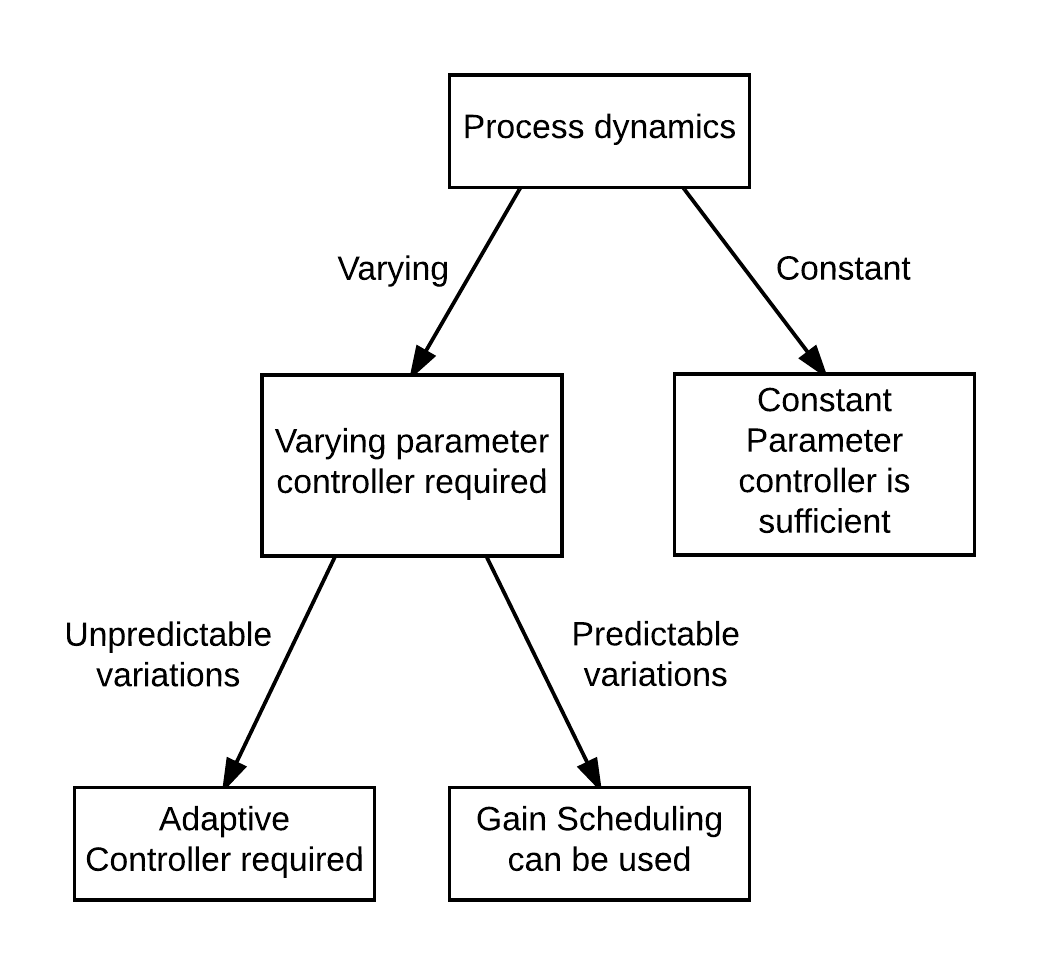
\includegraphics[width=0.85\textwidth]{why_adaptive_control.png}
  \caption{Determine if adaptive control should be used}
  \label{fig:why_adaptive_control}
\end{figure}


%---------------------------------------------------------
\section{MIT Rule}


%---------------------------------------------------------
\section{Lyapunov Stability Criteria}

Aerospace controllers tend to use linear controllers for their simplicity and well understood robustness characteristics.  This is despite the fact that the applications of these linear controllers are applied to a non-linear dynamical system such as attitude control with varying dynamic pressure.  Adaptive Controllers are non-linear and may offer performance benefits to non-linear systems as seen in aforementioned aerospace applications.  However, non-linear controller's robustness properties need to be evaluated.  The Lyapunov stability criteria offers methods of evaluating these controller's boundedness and robustness behavior.  

Aleksandr Lyapunov was a Russian mathematician who's work was published in 1892 \cite{lyapunov1892general} concerning the behavior of non-linear systems close to equilibrium without having to rigorously find the unique solutions to difficult differential equations used to model the system.  His work was largely overlooked until the Cold War when aerospace solutions required a more rigorous approach to analyzing non-linear control robustness.  Modern non-linear control engineers extensively utilize Lyapunov's techniques to design and evaluate non-linear controllers.

\subsection{Lyapunov Stability Definitions}

Lyapunov's methods attempt to evaluate autonomous nonlinear dynamical systems within the bounds of three classifications.  In this case the autonomous system is defined as definable set of ordinary differential equations which are not explicitly dependent upon the independent variable.  These classifications can be used to define a nonlinear system as Lyapunov stable, asymptotically stable, or exponentially stable.

Given the following autonomous nonlinear dynamical system:

 \begin{equation}
\dot{x}(t)=f(x(t)), \qquad x(0)=x_0
\end{equation}

where $f$ has equilibrium at $x_e$ :
 \begin{equation}
f(x_e) = 0
\end{equation}

then the equilibrium is said to be:
\begin{enumerate}
	\item \textbf{Lyapunov Stable} \newline
	for every $\epsilon > 0$ there exists a $\delta > 0$ such that, if \: $\norm{x(0) - x_e} < \delta$, then for every $t \geq 0$ we have 	$ \norm{x(t) - x_e} < \epsilon$	
	\item \textbf{Asymptotically Stable} \newline
	if the system is Lyapunov stable and there exists a $\delta > 0$ such that if \: $\norm{x(0) - x_e}  < \delta$, then $\displaystyle \lim_{t\to \infty} \norm{x(t)-x_e} =0$
	\item \textbf{Exponentially Stable} \newline
	if the system is asymptotically stable and there exists $\alpha > 0, \beta > 0, \delta > 0$ such that if $\norm{x(0)-x_e}<\delta$, then \:$\norm{x(t)-x_e} \leq \alpha \norm{x(0)-x_e} e^{-\beta t}$, for all $t \geq 0$
\end{enumerate}

Being Lyapunov stable infers that if a system is near equilibrium then it will indefinitely remain near equilibrium.  If the system if found to be asymptotically stable then it eventually will achieve equilibrium as $t\to \infty$ and being exponentially stable implies it reaches equilibrium even faster.

\subsection{Lyapunov's Second Method}
 
Lyapunov's second proposed method is also known as Lyapunov stability criteria.  This method offers a less tenuous method for evaluating mathematically non-ideal systems.  Lyapunov analysis of the linearized system around equilibrium can be cumbersome in the case where equilibrium is at the origin or the eigenvalues are purely imaginary.  In this case, the solutions can rapidly depart to infinity or approach zero with little perturbation to the eigenvalues.  Lyapunov's second method offers an alternative approach for classifying a systems stability using a concept that is similar to how energy is defined in classical dynamics.

Conceptually, Lyapunov's second method can be compared to evaluating the energy of a vibrating spring mass system.  The energy of the unforced spring mass system will dissipate energy due to friction and or damping etc.  This trend of energy leaving the system towards some 'attractor' is evidence of the system's stability characteristics and identifies that there will be some stable end state.  Like wise, Lyapunov's second method characterizes this with the use of a Lyapunov candidate function $V(x)$.  It is important to note that Lyapunov realized that the candidate function can be any function so as long as one candidate function is found in agreement with the stability criteria.  It is then said to be Lyapunov stable if any candidate equation is found and meets the stability criteria.  This means that it is only incumbent upon the engineer to find one candidate equation to meet the criteria.  This can be an iterative process of trying multiple energy like equations.  A common approach is to model the Lyapunov candidate equation as kinetic energy $(\frac{1}{2}u^2)$.  Lyapunov realized that characterizing the energy of a nonlinear system could be almost impossible for some cases, but this approach could prove stability without the rigorous knowledge of the true system's energy.

Lyapunov's second method defines a system as Lyapunov Stable for a system $\dot{x}=f(x)$ having an equilibrium point at $x=0$ where the Lyapunov candidate function $V(x):\mathbb{R}^n \rightarrow \mathbb{R}$ such that:
\begin{itemize}
	\item $V(x)=0$ if and only if $x=0$
	\item $V(x)>0$ if and only if $x\neq0$
	\item $\dot{V}(x)=\frac{d}{dt}V(x)=\sum\limits_{i=1}^{n} \frac{\partial V}{\partial x_i}f_i(x) \leq 0$, for all values of $x\neq 0$		
\end{itemize}

if $\dot{V}(x) < 0$ for $x\neq 0$ then system is asymptotically stable.

To determine if the system is globally stable, it is additionally required to prove the condition of radial unboundedness.










